\chapter{Auswahl der Hardware}

\section{Einleitung}
Die Auswahl von Hardware mit ARM Prozessoren ist extrem gross.
Ende September 2016 sind bereits über 86 Milliarden ARM basierte Prozessoren verkauft worden.\footnote{Elektronischer/Anhang/ARM-media-fact-sheet-2016.pdf}
Diese Zahl reflektiert zwar nicht direkt die Diversität von den verschiedenen Prozessoren, aber sie zeigt recht gut wie enorm weit ARM Prozessoren verbreitet sind.

In diesem Kapitel soll in dem riesigen Angebotsdschungel die richtige Hardware ausgewählt werden, auf der diese Arbeit aufbauen kann.
% Die ausgewählte Hardware soll ein Experimentierboard mit einem ARM-Prozessor gefunden werden, dass im Robotik Unterricht verwendet werden kann.
Die ausgewählte Hardware soll nicht nur für diese Arbeit genutzt werden, sondern auch für den Robotik Unterricht.
Zusätzlich sollte der Prozessor auch leistungsstark und auch flexibel genug sein, um ihn in anspruchsvollen Robotikprojekten verwenden zu können.
%TODO extrem weit verbreitet
%TODO gorosse auswahl von verschiedener hw
%TODO warum muss hw in dieser arbeit gewählt werden

%TODO prozeossor und board muss ausgewählt werden
%TODO ökosystem?

\section{Soll- und Muss-Kriterien bei der Auswahl der Hardware}
Für die Hardware sind folgende Soll- und Muss-Kriterien ermittelt worden.

\subsection{Muss-Kriterien}
\begin{itemize}
\item Systemebene
	\begin{itemize}
	\item FPGA: Der Prozessor muss mit einem FPGA kommunizieren können.
	\item Hardware Debugger: Der Prozessor muss für die Entwicklung von \textit{deep} einen Hardware Debugger wie beispielsweise das JTAG Interface BDI3000\footnote{http://www.abatron.ch/fileadmin/user\_upload/news/BDI3000-Brochure.pdf} von Abatron unterstützen. 
	\item Günstiger Programmierer: Wenn zusätzliche Hardware benötigt wird um die \textit{deep}-Applikation auf das Target zu schreiben, dann muss diese möglichst günstig sein.
	\item Grosses Ökosystem: Das ausgewählte Produkt muss von einem grossen Ökosystem unterstützt werden. Aussterbende Produkte oder Nischenprodukte sind nicht akzeptabel.
	\item Als fertiges Modul erhältlich: Eigenes PCB entwickeln und herstellen ist keine Option.
	%TODO synonym einbettbar:
	\item Einbettbar: Der Prozessor muss auch bei einem selbst entwickelten PCB verwendet werden können. Wahlweise als SOM (\textit{System On Module}) oder direkt als Prozessor in eigenem Package.
	\item Noch lange erhältlich.
	\end{itemize}
\item Prozessorebene
	\begin{itemize}
	\item ARMv7: Der Prozessor muss auf einer ARMv7 ISA (\textit{Instruction Set Architecture}) basieren.
	\item ARM Instruktionen: Der Prozessor muss ARM Instruktionen unterstützen. \textit{Thumb} Instruktionen sind nicht ausreichend.
	\item FPU (\textit{Floating Point Unit}): Für Gleitzahlenarithmetik.
	\item Netzwerkschnitstelle: RJ-45 inklusive MAC\footnote{Media Access Control} und \textit{Magnetics}.
	\item USB: USB Schnittstelle als Host und als Slave.
	\item Flash: Mehr als 50kByte Flash.
	\item RAM: Mehr als 100kByte RAM.
	\end{itemize}
\end{itemize}


\subsection{Soll-Kriterien}
\begin{itemize}
\item Systemebene
	\begin{itemize}
	%TODO synonym einbettbar:
	\item Einfach einbettbar: Der Prozessor ist als Prozessormodul erhältlich, so dass das Design von einem selbst entwickelten PCB einfacher wird.
	\item Günstiger Hardwaredebugger: Der Hardwaredebugger kann auch für Applikationsentwicklung mit \textit{deep} eingesetzt werden.
	\item Möglichst schneller Download der Applikation.
%TODO	\item Überdimensionierte HW
	\end{itemize}
\item Prozessorebene
	\begin{itemize}
	\item Memory Mapped Bus für FPGA Schnittstelle.
	\item FPU unterstützt \textit{Double Precision}.
	\item Integerdivision
	\item Prozessortakt über 500MHz.
	\end{itemize}
\end{itemize}


\section{Hardware Debugger}
Der Begriff \textit{Hardware Debugger} ist nicht eindeutig definiert.
Im einfachsten Fall kann ein Hardware Debugger nur ein \textit{Boundary Scan} durchführen wie es ursprünglich für JTAG vorgesehen war.
Bei \textit{Boundary Scan} können die I/O Pins von einem Prozessor gelesen und auch gesetzt werden.
Mit so einem Scan kann in der Produktion bei der Bestückten PCBs überprüft werden, ob alle Lötstellen Kontakt herstellen und dabei keine Kurzschlüsse bilden.
Für diesen Scan wird der Prozessor Kern nicht verwendet, sondern separate Peripherie im Prozessor.
Über das JTAG Interface kann der Scan ausgeführt werden, ohne dass eine Software auf dem Prozessor ausgeführt werden muss.

Moderne Prozessoren erweitern diese grundlegende Funktionen mit einigen sehr hilfreichen Features.
% Moderne Prozessoren haben noch viel mehr Funktionen.
So bieten ARM Prozessoren mit der \textit{CoreSight} Technologie noch viel mehr als nur einen \textit{Boundary Scan}.
% TODO besserer Satz
Die untenstehende Liste zeigt einige Funktionen von dieser Technologie, aber nicht alle.
Die für diese Arbeit relevanten Funktionen sind \textbf{fett} geschrieben.

\begin{itemize}
	\item \textbf{Prozessor Register lesen und schreiben}
	\item \textbf{RAM lesen und schreiben}
	\item \textbf{Externer Flash Speicher lesen und schreiben} 
	\item \textbf{Hardware Breakpoint auf den Program Counter} 
	\item \textbf{Hardwaer Breakpoint auf einer Speicherstelle (Watchpoint)} 
	\item Debug Trace (ETM Program Trace) 
	\item Debug Trace Buffer
\end{itemize}

Da ein Hardware Debugger keine funktionsfähige Software auf dem Prozessor benötigt, kann er auch gut verwendet werden, um die grundlegendsten Funktionen, wie beispielsweise der Bootvorgang, vom \textit{deep} Laufzeit System zu entwickeln.




\section{Übersicht über die ARM Mikroarchitekturen}
\subsection{Cortex-A}
Sehr gut geeignet für die Verwendung mit einem vollen Betriebssystem wie Windows, Linux oder Android.
Cortex-A Prozessoren bieten dem umfangreichsten Support für externe Peripherie wie USB, Ethernet und RAM.
Sie sind auch leistungsstärksten ARM Cortex Prozessoren.

\subsection{Cortex-R}
Cortex-R werden entwickelt für Echtzeitanwendungen und Sicherheitskritische Applikationen wie Festplattenkontrolle und medizinische Geräte.
Sie sind normalerweise nicht mit einer MMU \textit{Memory Management Unit} ausgerüstet.
% und können deshalb nich mit einem Linux oder Windows verwendet werden.
Mit einer Taktrate von über 1GHz und einem sehr schnellen Interruptverhalten eignen sich Prozessoren mit einem Cortex-R sehr gut um auf externe Stimuli schnell zu reagieren.

\subsection{Cortex-M}
Cortex-M sind mit einer Taktrate um 200Mhz relativ langsam.
Sehr stromsparend und durch die kurze Pipeline haben sie eine deterministische und kurze Interrupt Verzögerung.
Die Prozessoren aus der Cortex-M Reihe unterstützen nur die Thumb-Instruktionen und kommen deshalb nicht in Frage.


\subsection{ARM Prozessoren ausserhalb der Cortex Reihe}
Seit 2004 werden die meisten Kerne in eine der Cortex Gruppen eingeteilt.
Ältere Kerne, sogenannte \textit{''Classic cores''}, haben Namen wie z.b. ARM7 oder ARM1156T2F-S.
Da solche Designs meist aus einer Zeit vor 2004 stammen, gilt das Design als veraltet und wird bei dieser Arbeit nicht berücksichtigt.

\subsection{Fazit über die ARM Mikroarchitekturen}
Prozessoren die auf der Cortex-A Mikroarchitektur basieren bieten die grösste Flexibilität.
Zusätzlich ist auch das Angebot bei den Cortex-A Prozessoren am grössten.
Die anderen Cortex Reihen bieten keine Vorteile, die für dieses Projekt von Nutzen sind.
Aus diesen Gründen wird die Auswahl auf die Prozessoren aufs der Cortex-A Reihe begrenzt.

% TODO tabellen titel und referenz?
\begin{table}[]
\centering
\caption{Übersicht ARM Mikroarchitekturen}
\label{t-uebersichtARMMikroarchitekturen}
\begin{tabular}{|l|l|l|}
\hline
\textbf{}  & \textbf{Vorteile}                                                                                                                                                                                                                                    & \textbf{Nachteile}                                                                                                                                                                             \\ \hline
\textbf{A} & \begin{tabular}[c]{@{}l@{}}* Sehr Leistungsstark\\ * Support für vollwertige Betriebssysteme\\ * Grosse Variation erhältlich (Energiesparend /\\  sehr Leistungsstark)\\ * Reichhaltiger Funktionsumfang\\ * NEON und FPU Unterstützung\end{tabular} & \begin{tabular}[c]{@{}l@{}}* Langsamer Context-Switch\\ * Relativ hoher Stromverbrauch\\ * Relativ teuer\\ * Mit GPU erhältlich\\ * Keine DSP Unterstützung\\ * Keine HW-Division\end{tabular} \\ \hline
\textbf{B} & \begin{tabular}[c]{@{}l@{}}* Sehr gut geeignet für Echtzeitanwendungen\\ * Sehr schneller Context-Switch\\ * DSP Unterstützung\end{tabular}                                                                                                           & \begin{tabular}[c]{@{}l@{}}* Kleiner Funktionsumfang\\ * Nicht so leistungstark wie Cortex A\\ * Keine Linux Unterstützung\end{tabular}                                                        \\ \hline
\textbf{C} & \begin{tabular}[c]{@{}l@{}}* Sehr schneller Context-Switch\\ * Sehr energiesparend\\ * DSP Unterstützung\end{tabular}                                                                                                                                & \begin{tabular}[c]{@{}l@{}}* Geringe Rechenleistung\\ * Keine Linux Unterstützung\\ * Unterstützt nur Thumb-Instruktionen\end{tabular}                                                         \\ \hline
\end{tabular}
\end{table}



\section{Anbindung des FPGAs}
\subsection{Einleitung}
FPGAs haben typischerweise einen sehr hohen \textit{Pin-Count} und werden in \textit{BGA-Packages} ausgeliefert.

Es gibt verschiedene Möglichkeiten, wie ein FPGA mit einem Prozessor verbunden werden kann.
Die Vor- und Nachteile der verschiedenen Bauarten werden in diesem Kapitel abgewogen und im Bild \ref{fig:anbindungFPG} schematisch zusammengefasst.

% Um ein FPGA an einen Prozessor anzubinden kann eine serielle und auch parallele Kommunikation verwendet werden.


% % TODO zwei mal z.b.
% Ein moderner Prozessor ist ein sehr komplexes elektronisches Bauteil welches zusätzliche Peripherie für beispielsweise Stromversorgung und auch diverse I/Os.
% Die Ethernet Schnittstelle braucht neben der RJ-45 Buchse auch noch Signaltransformatoren, sogenannte Magneticts.
% % % TODO doofer satz
% % Auch wenn die Physikalische Anbindung der Ethernet Schnittstelle nicht ganz trivial ist, ist die Anbindung von RAM sehr viel anspruchsvoller.

% % Externer RAM muss über sehr viele Leitungen, welche alle gleich lang sein müssen und auch von der elektrischen Impedanz enge Parameter erfüllen müssen, an den Prozessor angeschlossen werden.
% % Diese Ansprüche erfordern sehr hohe Fachkenntnisse vom Designer.



\begin{figure}[htbp]
	\centering
		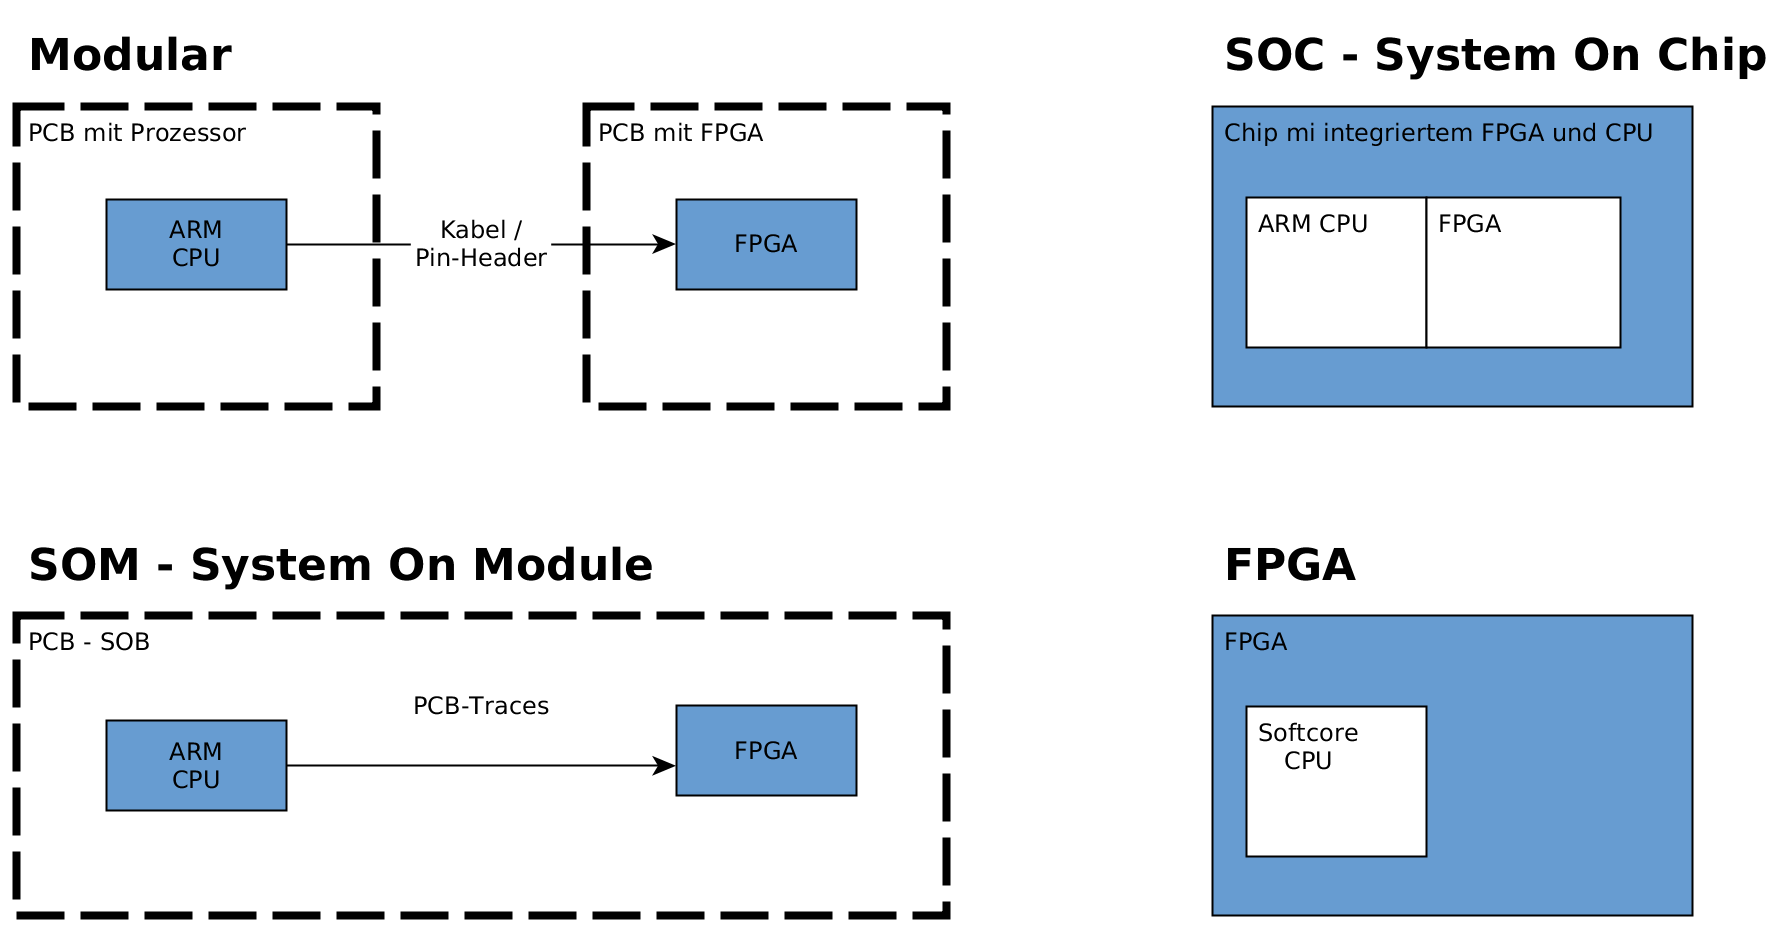
\includegraphics[width=\textwidth,height=\textheight,keepaspectratio]{graphs/bauformen.png}
	\caption[]{Mögliche Anbindungen des FPGA an die CPU}
	\label{fig:anbindungFPG}
\end{figure}
% \FloatBarrier


\subsection{FPGA als Zusatzplatine zum Prozessorboard - Bauweise ''Modular''}
Das \textit{FPGA Development Board CAPE for the BEAGLEBONE}\footnote{https://www.element14.com/community/docs/DOC-69215/l/fpga-development-board-cape-for-the-beaglebone} ist eine Aufsteckplatine für den \textit{Beaglebone Black}.
Wenn es auf den \textit{Beaglebone Black} aufgesteckt wird, erweitert es den ARM basierten Linux PC um \textit{Spatran 6 LX9} FPGA inklusive einiger I/O-Peripherie und SDRAM.

\textit{Vorteile:}
\begin{itemize}
	\item Relativ günstig.
	\item Funktioniert ''Out of the Box''
	\item Schnelles GPMC\footnote{General-Purpose Memory Controller} Interface (bis zu 70 MB/s) zwischen Prozessor und FPGA.
\end{itemize}

\textit{Nachteile:}
\begin{itemize}
	\item Verwendet ein modifiziertes Linux-Image, das LOGI-Image.
	\item Der eMMC\footnote{Embedded Multi Media Card} Speicher des Beaglebone kann nicht gleichzeitig mit dem GPMC verwendet werden.
	\item Die Verfügbarkeit vom Cape ist nicht garantiert.
	\item Nur ein FPGA und Prozessor erhältlich.
\end{itemize}

\textit{Fazit - Bauweise ''Modular''}
% unflexibel
%  - nur ein prozessortyp fpga
%  - custom pcb muss nachgebaut werden

\subsection{FPGA auf dem gleichen Modul wie der Prozessor (System On Module) - Bauweise ''SOM''}
Bei einem SOM (System On Module) ist die CPU und auch der FPGA auf dem gleichen PCB-Modul verbaut verbaut.
Dadurch ist eine sehr hohe Bandbreite bei der Kommunikation zwischen der CPU und dem FGPA möglich.
Das Modul benötigt ein zusätzliches PCB, ein Basisboard, in dem es eingebettet werden kann.
Oft existieren Experimentierboards mit einer grossen Zahl an unterschiedlichen I/O-Möglichkeiten die gebrauchsfertig gekauft werden können.
Für eine spezifische Anwendung muss so ein Basisboard für das SOM selbst designed werden, da ein Experimentierboard oft zu gross ist, oder nicht die benötigte Peripherie enthält.
Da neben dem FPGA auch High-Speed-Peripherie wie z.B. RAM auf dem Modul verbaut ist, kann beim Basisboard oft auf die aufwändige Entwicklung von High-Speed-PCB-Traces verzichtet werden.

Es hat sich gezeigt, dass nur eine Firma ein SOM mit FPGA produziert.
Die Firma XXX verkauft ein Module mit einem XXX Prozessor und einem XXX FPGA.

% TODO link für SOM

Da die Auswahl für SOMs sehr klein ist wurde diese Bauform nicht mehr weiter verfolgt.

 
\subsection{FPGA im gleichen Gehäuse wie der Prozessor (System On Chip - Bauweise ''SOC''}
Seit einigen Jahren werden Produkte verkauft, die eine programmierbare Logik (FPGA) und auch eine dedizierte CPU in einem Chip-Gehäuse verbaut haben.
Da der FPGA und auch die CPU im selben Gehäuse verbaut sind, ist eine sehr schnelle, integrierte Kommunikation zwischen CPU und FPGA möglich.
x

\subsection{ARM als Softcore in FPGA - Bauweise ''FPGA''}

% \subsubsection{Übersicht Bauformen}
\begin{table}[]
\centering
\caption{Übersicht Bauformen}
\label{t-uebersichtBauformen}
\begin{tabular}{|l|l|l|}
\hline
\textbf{Bauweise} & \textbf{Vorteile}                                                                                                                      & \textbf{Nachteile}                                                       \\ \hline
\textbf{Modular}  & \begin{tabular}[c]{@{}l@{}}* Günstig wenn nur Prozessor verwendet wird\\ * Unterschiedliche FPGAs können verwendet werden\end{tabular} & * Datenbus evt. nicht Memory mapped                                      \\ \hline
\textbf{SOB}      & \begin{tabular}[c]{@{}l@{}}* Sauberes, abgeschlossenes System\end{tabular} & * FPGA ist fix                                                           \\ \hline
\textbf{SOC}      & \begin{tabular}[c]{@{}l@{}}* Potenziell sehr schnelle Datenverbindung\\ \ \ \ zwischen FPGA und Prozessor\\ * Sauberes, abgeschlossenes System\end{tabular}                       & \begin{tabular}[c]{@{}l@{}}* FPGA ist fix\\ * Relativ teuer\end{tabular} \\ \hline
\textbf{FPGA}     & * Flexibel                                                                                                                             & * Sehr teuer                                                             \\ \hline
\end{tabular}
\end{table}

%\section{Cortex-M}
%\textbf{Cortex-M0}
%A very small processor (starting from 12K gates) for low cost, ultra low power microcontrollers and deeply embedded applications
%
%\textbf{Cortex-M0+}
%The most energy-efficient processor for small embedded system. Similar size and programmer’s model to the Cortex-M0 processor, but with additional features like single cycle I/O interface and vector table relocations
%
%\textbf{Cortex-M1}
%A small processor design optimized for FPGA designs and provides Tightly Coupled Memory (TCM) implementation using memory blocks on the FPGAs. Same instruction set as the Cortex-M0
%
%\textbf{Cortex-M3}
%A small but powerful embedded processor for low-power microcontrollers that has a rich instruction set to enable it to handle complex tasks quicker. It has a hardware divider and Multiply-Accumulate (MAC) instructions. In addition, it also has comprehensive debug and trace features to enable software developers to develop their applications quicker
%
%\textbf{Cortex-M4}
%It provides all the features on the Cortex-M3, with additional instructions target at Digital Signal Processing (DSP) tasks, such as Single Instruction Multiple Data (SIMD) and faster single cycle MAC operations. In addition, it also have an optional single precision floating point unit that support IEEE 754 floating point standard
%
%\textbf{Cortex-M7}
%High-performance processor for high-end microcontrollers and processing intensive applications. It has all the ISA features available in Cortex-M4, with additional support for double-precision floating point, as well as additional memory features like cache and Tightly Coupled Memory (TCM)



\subsubsection{STM23}
STM